\documentclass[BTech]{iitmdiss}
\usepackage{times}
\usepackage{epsf}
\usepackage{threeparttable}
\usepackage{float}
\usepackage{setspace}
\usepackage{amsmath}
\usepackage{amsthm}
\usepackage{txfonts,pxfonts,amsfonts}
\usepackage{epsfig}
\usepackage{caption}
\usepackage{subfig}
\usepackage{graphicx}

% \usepackage[square,numbers,sort]{natbib}
\usepackage[square]{natbib}
\usepackage[hypertex]{hyperref} % hyperlinks for references.
%\usepackage{algorithmic}
%\usepackage{algorithm}


%\include{commands}

% Strut macros for skipping spaces above and below text in tables. 
\def\abovestrut#1{\rule[0in]{0in}{#1}\ignorespaces}
\def\belowstrut#1{\rule[-#1]{0in}{#1}\ignorespaces}

\def\abovespace{\abovestrut{0.20in }}
\def\aroundspace{\abovestrut{0.20in}\belowstrut{0.10in}}
\def\belowspace{\belowstrut{0.10in}}
%%%%%%%%%%%%%%%%%%%%%%%%%


\def\thesistitle{Telemetry / Telecommand Frontend - IITMSAT}
\def\thesisauthor{Anoop R Santhosh}


\begin{document}
\bibliographystyle{iitm}
%%%%%%%%%%%%%%%%%%%%%%%%%%%%%%%%%%%%%%%%%%%%%%%%%%%%%%%%%%%%%%%%%%%%%% 
% Title page

\title{\thesistitle}

\author{\thesisauthor}

\date{May 2014}
\department{Computer Science and Engineering}

%\nocite{*}
\begin{singlespace}
\maketitle 
\end{singlespace} 



%%%%%%%%%%%%%%%%%%%%%%%%%%%%%%%%%%%%%%%%%%%%%%%%%%%%%%%%%%%%%%%%%%%%%%
% Certificate
\certificate

\vspace*{0.5in}

\noindent This is to certify that the thesis entitled {\bf {\thesistitle}}, 
submitted by {\bf {\thesisauthor}}, to the Indian Institute of Technology, 
Madras, for the award of the degree of {\bf Bachelor of Technology}, 
is a bona fide record of the research work carried out by him under my
supervision. The contents of this thesis, in full or in parts, have not been
submitted to any other Institute or University for the award of any degree or
diploma.

\vspace*{1.4in}
\hspace*{-0.25in}
\begin{singlespace}
\noindent {\bf Dr.~Shankar.~Balachandran } \\
\noindent Project Guide \\ 
\noindent Assistant Professor \\
\noindent Dept. of Computer Science and Engineering\\
\noindent IIT-Madras, 600 036 \\
\end{singlespace}
\vspace*{0.20in}
\noindent Place: Chennai\\ 
Date:

%%%%%%%%%%%%%%%%%%%%%%%%%%%%%%%%%%%%%%%%%%%%%%%%%%%%%%%%%%%%%%%%%%%%%%
% Acknowledgements
\acknowledgements

I would like to express my special appreciation and thanks to my advisor Dr. Shankar Balachandran for his inspiration, support and guidance throughout this project and entire 4 years in general. He is a great teacher and a tremendous mentor.
\par I would also like to thank Dr. Harishankar Ramachandran, for the time he devoted towards discussing the design and motivating me in general.
\par My sincere thanks also goes to Dr. David R. Koilpillai, for his invaluable feedback and the inspiring talks during every IITMSAT session.
\par I would like to extend my gratitude to Mr.Akshay Gulati, the person who motivated me to join IITMSAT team . He has been a wonderful mentor , devoting a lot of his time discussing the design and implementaion.

\par I am grateful to the entire Computer Science Department ,IITMSAT team and my batchmates for their support.

\par Last, but not least , I am grateful to my parents and friends for their constant support and motivation. 

%%%%%%%%%%%%%%%%%%%%%%%%%%%%%%%%%%%%%%%%%%%%%%%%%%%%%%%%%%%%%%%%%%%%%%
% Abstract

\abstract

\noindent KEYWORDS: \hspace*{0.5em} \parbox[t]{4.4in}{TMTC FrontEnd,
AX.25, IITMSAT}

\vspace*{24pt}

IITMSAT is a low orbit nano satellite being developed by students at IIT Madras. The satellite project has various subsystems, both hardware and software . Ground station software is an important part of it. TMTC Frontend is an important sub module within the ground station software. It essentially functions as the link layer and implements the link layer protocol which in this case is AX.25 .
\par The main functionality of this module includes AX.25 protocol encoding/decoding , flow control including acknowledgements and counters and packet reassembly. The overall design is loosely inspired by the SwissCube ground station design. But to satisfy IITMSAT mission requirements which are different from SwissCube, many modifications were made, especially in the telecommand transmitter part. The link layer protocol though based on standard AX.25 protocol, has been modified to meet our requirements. 


\pagebreak

%%%%%%%%%%%%%%%%%%%%%%%%%%%%%%%%%%%%%%%%%%%%%%%%%%%%%%%%%%%%%%%%%
% Table of contents etc.

\begin{singlespace}
\tableofcontents
\thispagestyle{empty}

%\listoftables
%\addcontentsline{toc}{chapter}{LIST OF TABLES}
\listoffigures
\addcontentsline{toc}{chapter}{LIST OF FIGURES}
\end{singlespace}


%%%%%%%%%%%%%%%%%%%%%%%%%%%%%%%%%%%%%%%%%%%%%%%%%%%%%%%%%%%%%%%%%%%%%%
% Abbreviations
\abbreviations
 
\noindent 
\begin{tabbing}
xxxxxxxxxxx \= xxxxxxxxxxxxxxxxxxxxxxxxxxxxxxxxxxxxxxxxxxxxxxxx \kill

\textbf{CCSDS} \> Consultative Committee for Space Data System  \\
\textbf{CRC} \> Cyclic Redundancy Check \\
\textbf{ECSS} \> European Cooperation for Space Standardization \\
\textbf{GS} \> Ground Station \\
\textbf{ISRO} \> Indian Space Research Organisation \\
\textbf{MCS} \> Mission Control System \\
\textbf{MDR} \> Mission Data Repository \\
\textbf{MIB} \> Mission Information Base \\
\textbf{SDR} \> Software Designed Radio \\
\textbf{SSID} \> Secondary Station Identifier \\
\textbf{TC} \> Telecommand \\
\textbf{TM} \> Telemetry \\
\textbf{TMTC} \> Telemetry \ Telecommand \\
\textbf{VC} \> Virtual Channel \\

\end{tabbing}

\pagebreak

%%%%%%%%%%%%%%%%%%%%%%%%%%%%%%%%%%%%%%%%%%%%%%%%%%%%%%%%%%%%%%%%%%%%%%
%Notation

% \chapter*{\centerline{NOTATION}}
 %\addcontentsline{toc}{chapter}{NOTATION}
 
 %\begin{singlespace}
 %\begin{tabbing}
 %xxxxxxxxxxx \= xxxxxxxxxxxxxxxxxxxxxxxxxxxxxxxxxxxxxxxxxxxxxxxx \kill
 %\textbf{$r$}  \> Radius, $m$ \\
 %\textbf{$\alpha$}  \> Angle of thesis in degrees \\
 %\textbf{$\beta$}   \> Flight path in degrees \\
 %\end{tabbing}
 %\end{singlespace}
 
 %\pagebreak
 %\clearpage

%The main text will follow from this point so set the page numbering
%to arabic from here on.
\pagenumbering{arabic}


%%%%%%%%%%%%%%%%%%%%%%%%%%%%%%%%%%%%%%%%%%%%%%%%%%
% Introduction.

 \chapter{INTRODUCTION}
 \label{chap:intro}
 
\par This chapter provides a brief introduction to IITMSAT in general and the particular problem statement i.e, TMTC Frontend .
 
 \section{An introduction to IITMSAT }
 IITMSAT is a student initiated  satellite project being developed at IIT Madras. The project mission is to launch a nano satellite into a low earth orbit of altitude 600 - 1000 km .The orbit passes through the mission's region of interest, the ionosphere. Being an auxillary satellite on the launch vehicle, IITMSAT does not have prior control over the exact altitude. IITMSAT is proposed to carry an on-board High Energy Particle Detector (HEPD) and measure changes in charged particle flux in the upper ionosphere. Data gathered by HEPD, including orientation, time, position of the satellite and flux data is referred to as Science Data (SC). SC data will be stored on the on-board memory of the satellite. Besides HEPD, satellite has various sensors on-board to monitor parameters like temperature, current, voltage etc. This data is referred to as Housekeeping (HK) data.
 \par Both HK data and SC data are transmitted to the ground station when the satellite comes in the field of view. IITMSAT proposes to have just one ground station set up in the IIT Madras campus. The ground station will receive both HK data and SC data. HK data will be used to monitor the health of the satellite whereas SC data will be analyzed by the ground station software and displayed to users in human interpretable formats.  


The main configurations/features of the satellite are as given below:
\begin{itemize}

\item \textbf{Orbit : } Low earth Orbit
\item \textbf{Altitude : } 600 km to 800 km
\item \textbf{Inclination : } \textgreater  45 degrees 
\item \textbf{Mission Life Time : } \textgreater 1 year 
\item \textbf{Dimensions : }  29 cm x 29 cm x 26 cm
\item \textbf{Mass : } 15 kg
\item \textbf{Payload : } High Energy Particle Detector 
\end{itemize}
 
 \section{An overview of Ground Station software}
 Ground station software is responsible for handling the operations of the satellite from ground and process the information transmitted by the satellite on down-link.It provides an interface for interacting with satellite and analyzing data besides keeping track of various parameters of the satellite.The major modules within the ground station software are : 
 
 \begin{itemize}
 \item \textbf{User Interface : }UI allows human users to select commands to control the satellite. It also displays various data collected by the satellite payload and housekeeping data after processing it in appropriate ways.
 \item \textbf{Mission Control System }: MCS is responsible for converting the user input to CCSDS telecommands before dispatching them to the satellite . It is also responsible for archiving all packets sent and received. It is also the unit which schedules commands and processes the data received from satellite (CCSDS packets ) on downlink. It interacts with UIs on one end and TMTC Frontend on the other. It transmits and receives CCSDS packets to/from TMTC Frontend.
 \item \textbf{TMTC Frontend : } This layer acts as a link layer for communication between MCS and satellite. Functionalities of TMTC Frontend are mentioned briefly in the next section on problem statement. Chapter 2 explains more details of the working of this layer.  
 \end{itemize}

 \section{TMTC Frontend - The problem statement}
The main problem statement is to implement a robust TMTC Frontend. TMTC Frontend is the layer between MCS and GS hardware. It acts as a link layer for communication between GS and satellite . It is expected to provide the following functionalities :
\begin{itemize}
\item \textbf{Up-link : } 
\begin{itemize}
\item Encoding CCSDS packets (telecommand) to AX.25 frame.
\item Archive AX.25 telecommand frames.
\item Flow Control (resending, counters, acknowledgments etc ).

\end{itemize}
\item \textbf{Down-link : }
\begin{itemize}
\item Decode AX.25 frame (telemetry) and reassemble the application data to obtain CCSDS packets.
\item Archive raw AX.25  telemetry frames. 

\end{itemize}
\item \textbf{Replay : }
\begin{itemize}
\item Provide functionality to replay archived raw AX.25 telemetry frames.
\end{itemize}
\end{itemize}
TMTC Frontend is explained in more detail in chapter 2. 
 
 \section{Motivation}
 
A robust link layer is very essential for proper communication with the satellite. This layer is responsible for encoding application data (CCSDS packets) to AX.25 protocol on up-link and decoding  AX.25 frames to CCSDS packets on down-link. There are two major concerns about the communication link with the satellite which necessitates a robust link layer. One concern is the reliability of the communication link to the satellite. Being an  satellite, it is not feasible for IITMSAT to have a professionally competent communication system. This combined with various external interferences like radiation effects and other space environment effects can reduce the reliability of the link. Another major concern is the limited time available to communicate with the satellite. As mentioned earlier IITMSAT proposes to have only one ground station. During each pass GS gets a communication window of around 8 minutes. With just one GS, only two to three passes can be expected in a day. This gives a communication window of roughly around 16 - 24 minutes in a day. Maximum data transfer should be ensured within this limited time. 
\par A robust link layer is essential to counter the effects of limited link reliability and communication time.The link layer should be able to handle acknowledgments and resending of dropped packets automatically without involving the application layer. Once the application layer (in IITMSAT case ,MCS) is involved in flow control like acknowledgments, resending etc, it can slow down operations and affect the amount of data transferred. Since all data/command transfer between MCS and satellite happens through this layer, failure of this layer can cut off communication with the satellite.

\section{SwissCube - a similar satellite mission}
SwissCube is CubeSat class satellite launched and operated by Ecole Polytechnique Fédérale de Lausanne (EPFL), Switzerland. A CubeSat is a miniaturized satellite of volume one liter which is usually used for space research. It was launched a Polar Satellite Launch Vehicle in 2009. It was expected to last three to twelve months, but the mission was extended for an additional 18 months.
When IITMSAT project was initiated in 2010, the initial design and model was largely influenced by SwissCube. As the IITMSAT project matured, it has evolved much more than SwissCube project in terms of mission specifications. Still IITMSAT design, atleast at a high level is heavily based on SwissCube. A lot of terminology and organization details used within IITMSAT project has been derived from SwissCube model.
Though there are marked differences in the implementation of ground station software of IITMSAT compared to SwissCube, the high level design is still influenced by SwissCube . The organization of UI, MCS, TMTC Frontend etc are based on the SwissCube design.  Though a discussion on the details of SwissCube is beyond the scope of this document, certain similarities and differences are mentioned at places where it is deemed necessary.  
\section{Contributions of this work}
Though the design is loosely based on GS software design of SwissCube, there are quite a few differences. The transmission of data was not a big concern in case of SwissCube, which is not the case with IITMSAT. Hence in SwissCube GS software, resending dropped frames is handled at MCS through manual control. However, in case of IITMSAT, we expect to transmit more commands/ data in uplink and cannot depend on manual control for frame retransmission. So our design involves automated retransmission at link layer itself, instead of involving application layer. 
\par Another major difference from SwissCube is that we have modified the AX.25 frame to support 256 outstanding telecommand frames at a time where as SwissCube design allows only for 4. Owing to the manual control over packet transmission , 4 outstanding packets were sufficient for SwissCube. But this is not the case with IITMSAT. 
\par IITMSAT TMTC Frontend ensures minimal human interference in frame transmission as opposed to SwissCube. This ensures faster and more reliable communication with the satellite. All the expected features of TMTC Frontend mentioned in the problem statement were implemented. Modified AX.25 protocol encoding/decoding library was implemented. A new telecommand transmitter was designed and implemented. Telemetry receiver was also implemented .Reassembly unit was implemented to support large data transfer. Archiving support for both telecommand and telemetry frames was implemented with a SQL database. Replay functionality was also implemented and a small GUI was created for replay controller.  Finally all the sub-modules were integrated together to build a robust TMTC Frontend, which was tested using simulations of MCS and GS hardware. 
 
 \section{Organisation of report}
 
This report is organised into 6 chapters. Chapter 2 explains a few terminology involved and frame structure of the protocols used. Chapter 3 gives a detailed explanation of the design of TMTC Frontend. Chapter 4 discusses  implementation details . Chapter 5 explains how the software system was tested. Chapter 6 is the Conclusion chapter . 

 \chapter{BACKGROUND DETAILS}
 \label{chap:background}
This chapter gives a brief background on IITMSAT ground station software and detailed specifications of TMTC Frontend .
\section{Ground Station Software}
As briefly mentioned in the introduction, ground station software is responsible for providing an interface to interact with the satellite and control the operations of the satellite from ground. The main user requirements are :
\begin{itemize}
\item Control the satellite and monitor its operations.
\item Process the downlink data and provide payload data in human interpretable format.
\item Monitor various house keeping parameters like voltage and alert users in case of an issue or takes action whenever possible.
\item A GUI for easy human interaction.
\item Implement application layer protocols in compliance with ECSS standards. CCSDS packets are used for application data encoding. 
\item Provide a reliable communication channel to the satellite. 
\end{itemize}

\begin{figure}[H]

\includegraphics[scale = 0.7]{gs.eps}
\caption{Ground Station software block diagram}
\label{fig:gs}
\end{figure}
Note : Within the CCSDS packet telemetry and telecommand concept
, an on-board application process is defined as the source of telemetry source packets and the sink for telecommand packets \citep{ecss}.Throughout this report telecommand refers to commands send to the satellite from GS and telemetry refers to data received by GS from the satellite.

A human user interacts with the ground station software through various graphical user interfaces. There are different GUIs like Mission Configuration Client, Telecommand Manager, Monitoring Data Display Client etc. Mission Control System (MCS) is responsible for handling user inputs from the GUI. 
\par During telecommand operations (uplink), the user selects telecommands for giving instructions to the satellite. The CCSDS encoding for all the telecommands are defined in Mission Information Base (MIB) which is a part of MCS. All telecommand and telemetry packet encoding are defined in MIB. After encoding information into CCSDS packets, these packets are packets are dispatched to TMTC Frontend for transmitting to the satellite. TMTC Frontend as mentioned earlier is the link layer. It encodes the CCSDS packets received from MCS into AX.25 telecommand frames. TMTC Frontend archives the frames and based on the flow control mechanism, transmits the frames to the satellite. TMTC Frontend drops off AX.25 telecommand frames to the Software Defined Radio (SDR) module in IITMSAT case. An SDR is used to implement hardware components of a typical radio communication system by means of software. GNU Radio is the SDR used by IITMSAT. SDR interacts with hardware components rather than TMTC Frontend. The GS hardware then transmits packets over a RF link to the satellite, which receives it and processes accordingly. 

\par During telemetry operations (downlink), the satellite transmits AX.25 telemtry frames through the RF link, which is the received by GS hardware and passed on to SDR. SDR after processing the frames, transfers them to TMTC Frontend. AX.25 frames are decoded and reassembled to obtain CCSDS packets at TMTC Frontend. It also archives ras AX.25 telemetry frames in an SQL database. If the received frame is an acknowledgement frame, it is passed to the telecommand transmitter. Otherwise the reassembled CCSDS packets are transferred to the MCS. MCS processes the CCSDS frames with the help of encodings defined in MIB. It then displays the information to the human user through the GUI. It also monitor the health of the satellite from housekeeping data.  

\par Besides this MCS also  contains another data repository called Mission Data repository (MDR). All telecommands and telemetry which passes through the MCS is archived in MDR. Planning tool and scheduler are not a very essential component of GS software. They can be used for intelligent planning and scheduling of communication with the satellite so as to ensure efficient communication.

\par The overall design of IITMSAT GS is inspired by the SwissCube GS, though the design of each component is not exactly similar to SwissCube.  

\section{TMTC Frontend}
TMTC Frontend as mentioned earlier acts a link layer between MCS and satellite.It handles protocol eencoding.decoding, flow control, reception and transmission of frames etc.

\begin{figure}[H]
\includegraphics[scale = 0.6]{tmtc.eps}
\caption{TMTC Frontend Block Diagram}
\label{fig:tmtc}
\end{figure}


\textbf{Uplink : }During uplink or telecommand transmission operations, TMTC Frontend receives CCSDS packets from MCS. These packets are encoded into modified AX.25 telecommand frames. The protocol frame structure is explained in next chapter. After it the packets are encoded to CCSDS frames, they are added to a transmission queue. The frames are also archived in a SQL database. The flow control mechanism described in next chapter handles the transmission of the frames from that point. When the conditions are suitable for dispatch of the packet, the transmitter drops off the AX.25 frames to the GNU radio module. GNU radio handles rest of the communication with the satellite.


\par\textbf{Downlink : }During downlink or telemetry reception operations, TMTC Frontend receives AX.25 telemetry frames from GNU Radio. Receiver checks for bit stream errors with a CRC check and then the byte array is parsed to obtain various field of the AX.25 telemetry frames. The source and destination addresses are checked to ensure the validity of the frame. Legitimate frames are then archived and forwarded to appropriate reassembly unit. Reassembly unit reassembles CCSDS packets from different frames and when a CCSDS frame is completely reassembled, it is forwarded to the MCS.

\linebreak
\linebreak
\textbf{Replay : }As mentioned above, all raw AX.25 frames received by the telemetry receiver is archived in an SQL database. Replay functionality allows the user to replay those frames. The users through a GUI can select frames which were received in a time range and simulate the frame reception that happened in that time range. This is useful when some module like MCS fails and we want to simulate operations again. Replay controller retrieves frames from the database and creates a reassemby unit which reassembles CCSDS packets and forwards them to MCS. 
\section{Link Budget }
As mentioned earlier, communication link with the satellite may not be extremely reliable. Hence the link should be modeled properly. However such a communication link can be affected by many factors like radiations, ionospheric charged particles etc. For modeling such a communication link, a complex set of parameters need to be considered. Hence rather than creating a model of our own, we have decided to use the SwissCube estimates. Since the altitude and parameters of both satellites are quite similar, this would be a good approximation. The bandwidth according to SwissCube model is 1200 bits/sec and error rate in  7\%. 
\chapter{COMMUNICATION PROTOCOL}
This chapter briefly discusses the link layer communication protocol used by IITMSAT. 
\section{Standard AX.25 protocol}
AX.25 is a data link layer protocol derived from X.25 protocol suite and designed for use by amateur radio operators\citep{ax25}. AX.25 is most frequently used to establish direct point to point links.SwissCube uses their own modified version of AX.25. Since the overall IITMSAT design is based on SwissCube design, IITMSAT has decided to use AX.25 frames modified to meet our needs. Most of the fields of the standard frame structure are useful for IITMSAT.  

\par There are generally three types of AX.25 frames:
\begin{itemize}
\item  \textbf{Information Frame : }Used for data transfer.
\item \textbf{Supervisory Frame : }Used for supervisory link control.
\item \textbf{Unnumbered Frame : } Provides additional control over the link.
\end{itemize}
These frames can be distinguished by the value of control field. A discussion on full features of the standard protocol is not necessary for understanding of our system . Hence it is omitted from this document. For more details on the protocol, refer ~\citep{ax25}. 

\section{Modified AX.25 frame structure for IITMSAT }
The protocol and acknowledgement mechanisms which comes with the standard AX.25 protocol does not suit our needs. For example , the protocol allows for only 8 outstanding packets, while our system needs more than 8 out standing packets.

\par We have decided to use only the frame structure of AX.25 protocol for our system and not the flow control mechanism described by the protocol. We have modified even the frame structure to suit our needs by adding extra fields and changing the interpretation of some fields (from the standard protocol ).We are just using the frame encoding with our modifications and not any other standard features of the protocol. For the sake of convenience this modified version will still be referred to as AX.25 protocol/frame throughout this document. 
\par  The modified frame structure is briefly described below. The header and trailer common for both telecommand and telemetry will be discussed first, followed by modifications specific to each of them.

\subsection{Modified AX.25 Frame }
The frame structure is as shown below : 
\newline
\begin{figure}[H]

\includegraphics[scale = 0.65]{ax25main.eps.eps}
\caption{AX.25 Transfer Frame Format.Adapted from ~\cite{ax25}}
\label{fig:AX25mainframe}
\end{figure}
\\Few important  fields are briefly explained below :
\begin{itemize}
\item \textbf{Flag : } A flag field is used to delimit the frames and occurs at both beginning and end. It is 8 bits long and has value 01111110 (0x7E) . To ensure that the flag sequence does not appear anywhere else in the frame, bit stuffing is done. A '0' bit is interested after 5 continuous '1' bits.
\item \textbf{Destination and Source Address : } Both have similar structure and length of 56 bits. Destination and Source represent satellite or ground station depending on whether it is uplink or downlink. The address field structure is given below:
\newline
\begin{figure}[H]

\includegraphics[scale = 0.65]{addressfield.eps}
\caption{AX.25 Address Field.Adapted from ~\cite{ax25}}
\label{fig:ax25addressfield}
\end{figure}

\\
\begin{itemize}

\item \textbf{CallSign : } 6 upper case letters.They are placed in C1 to C6 fields.
\item \textbf{SSID : } 4 bit integer used to identify multiple stations using the same call sign . They are placed in fields 3 to 6, with fixed values for other fields.
\end{itemize}
\item \textbf{Control bits : }8 bits long. Originally used to differentiate between the types of frames mentioned above, we no longer use it in our version. It is assigned a fixed value of 00000011 (0x03). This actually refers to an unnumbered frame. 
\item \textbf{Protocol Identifier : }8 bits long.Originally used to represent the layer 3 protocol used, we have modified this field to indicate if a frame is an acknowledgement frame or not. Value 00000011(0x03) indicates that it is an acknowledgement frame. Otherwise value is 11110000(0xF0), which as per standard protocol indicates no layer 3 protocol implemented.
\item \textbf{Frame Check Sequence : }CRC-CITT is used to calculate a 16 bit CRC. The polynomial used is x^{16}+x^{12}+x^{5}+1.A CRC check is essential for error detection after the frame reception. A frame is accepted only after a CRC check.  


\end{itemize}

\subsection{Telecommand Information Field Usage }

In case of telecommands, the only extra support needed is a frame counter of limit more than 8. To number the frames , the first byte of the information field is used as a  frame counter. Thus we have a modulo 256 counter for frames. Rest of the information field carries telecommand data , with a maximum size of 2040 bits or 255 bytes.Virtual channels are not supported on uplink.

\subsection{Telemetry Information Field Usage }
Telemetry information field has much more modifications than telecommand. An extra header and trailer are added. This is because on the top of providing a modulo 256 counter, support for virtual channels and large data transfer has to be provided. Virtual channels and large data transfer are discussed in detail in chapter 4.  The information field structure is given below: 
\newline
\begin{figure}[H]
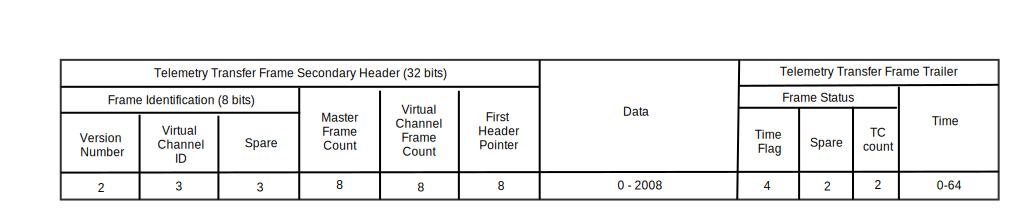
\includegraphics[scale = 0.5]{ax25telemetry.eps}
\caption{AX.25 Telemetry Header and Trailer }
\label{fig:ax25telemetry}
\end{figure}
\subsubsection{Secondary Header (32 bits) }
The secondary header is 32 bits long. It provides support for virtual channels and large data transfer (which will be discussed in detail later). The important fields are :
\begin{itemize}
\item \textbf{Frame Identification }
\begin{itemize}
\item Version Number (2 bits ) : Fixed to zero (00).
\item Virtual Channel ID (3 bits ) : Supports upto 8 virtual channels. Eg. 111 - represents data belongs to channel 8.
\item Spare (3 bits) : Reserved for future use. Value set to 000.
\end{itemize}
\item \textbf{Master Frame Count (8 bits)} : Total frame counter , ie., irrespective of the virtual channel. (modulo 256 counter).
\item \textbf{Virtual Channel Frame Count (8 bits ) }: Counter for a particular virtual channel (which corresponds to the current channel) . (modulo 256 counter ).
\item \textbf{First Header Pointer (8 bits) }: Specifies the octet number within the data field that contains the first octet of the first packet header.This allows the reassembly of packets even when previous packets were lost.
It has value 11111111(0xFF) if no packet header starts in the frame.


\end{itemize}
\subsubsection{Information Field(0 - 2008 bits)}
CCSDS packets are carried by the information field. It has a maximum length of 2008 bits.
\subsubsection{Trailer (0 to 72 bits ) }
\begin{itemize}
\item \textbf{Frame Status (8 bits) }
\begin{itemize}
\item \textbf{Time flag (4 bits) : } Gives size of time field. 000 indicates no time field. If bit 0 is set to 1, bits 1 to 3 indicate the size of time field in octets + 1.
\item \textbf{Spare (2 bits ) :} Reserved for future application. Set to 00.
\item \textbf{TC Counter (2 bits ) :} No longer used in the modified version. Set to 00.

\end{itemize}
\item \textbf{Time (0 - 64 bits ) : }On Board time . Represents the time at which end flag of previous frame was transmitted.
\end{itemize}

\subsection{Acknowledgement Frame }
As mentioned earlier, a frame is identified as acknowledgement frame by the value 0x03 in the protocol identifier field. All other fields like source and destination addresses, control bits etc are same as any other AX.25 frame. Individual packet numbers (acknowledgments), each a byte long are placed sequentially in the informtaion field. An acknowledgement frame does not contain a counter (for telecommand) or a telemetry header and trailer.

 \chapter{DESIGN OF TMTC FRONTEND}
 \label{chap:design}
 The TMTC Frontend consist roughly of four major sub modules.
\begin{itemize}
\item AX.25 Packet encoding/decoding
\item TC Transmitter
\item TM Receiver
\item Replay Controller
\end{itemize}
\section{AX.25 Packet encoding / decoding }
The frame structures of modified AX.25 protocol used by IITMSAT was discussed in the previous chapter.
This module implements a library to support encoding /decoding modified AX.25 protocol. A class is defined for the AX.25 frame which implements the common header. From this class, two classes are inherited for telecommand and telemetry frames. These classes implement fields specific to telecommand and telemetry. An AX.25 frame object can be created by either specifying values of each field or passing a byte array which is parsed to fill in each field. AX.25 frame classes (both telecommand and telemetry) has functions which return byte array representation of the frame. Implementation details of this module are discussed in next chapter. 

\section{TC Transmitter}
The telecommand transmitter is based on a state machine.Initially it was decided to use to the SwissCube transmitter algorithm. However it was quite limited for our requirements.
\subsection{Limitations of Swiss cube design}
The amount of telecommand packet transmission expected by SwissCube is lesser than what is expected by IITMSAT. The following features of SwissCube telecommand transmitter acts as a hindrance for adopting it in IITMSAT.
\begin{itemize}
\item It can support only 4 outstanding packets.
\item Packets are transmitted one at a time.
\item Transmission of packets are manually controlled by the user through MCS.
\item There was no option of resending at TMTC Frontend layer.
\item In the event of packet drop, the information is carried back to the application level, where a human user decides to resend the packet again.
The manual control, lack of automated resending and support for fewer outstanding packets can severely restrict the amount of telecomand which can be transmitted efficiently. 

\end{itemize}

\subsection{Modified Design}
The limitations mentioned above were not really a hindrance for operation of SwissCube. However, since IITMSAT expects more data transfer, it can be a serious concern. It slow down the number of frames transmitted . This is especially important as IITMSAT plans to have only one ground station. This severely restricts the amount of time a communication link can be opened with the satellite as it comes into the field of view for a short time every day.Hence we modified the design to support more outstanding packets and support for automated resending of frames at TMTC layer. The main characteristics are :
\begin{itemize}

\item All the packets in the ready queue are dispatched at the same time one after another. The number of packets is expected to be in the order of 10, which is way less than the 256 outstanding packets allowed.
\item Transmitter is half duplex. So we are not implementing an explicit timeout. Acknowledgement for a frame sent in a transmitter period is expected to come in the immediate next receiver period.
\item If acknowledgement is not received in the immediate next reception, packet is resent.A packet will be resent a fixed number of times, after which packet drop will be announced to MCS.

\end{itemize}

The states are :
\begin{itemize}
\item READY : Indicates that the transmitter is on and is ready to transmit frames. Positive beacon is the trigger to transmit frames.
\item WAIT\_FOR\_ACK : Indicates that the transmitter state machine is waiting for acknowledgement. 
\item WAIT\_FOR\_TRANS :  Indicates that the transmitter state machine is waiting for the physical transmitter to switch on. 
\end{itemize}

The external triggers are :
\begin{itemize}
\item Transmitter ON : Indicates switch to transmission mode.
\item Transmitter OFF : Indicates switch to reception mode.
\item Positive Beacon : Indicates that satellite is in field of view and ready for reception.
\item Ack received : Indicates the reception of acknowledgement packet by receiver.

\end{itemize}
The state diagram is as given below :
\begin{figure}[H]
\includegraphics[scale = 0.5]{state.eps}
\caption{TC Transmitter State Diagram }
\label{fig:state}
\end{figure}

\par When the transmitter state machine is in ready state, it is switched on and the a positive beacon trigger indicates that satellite is ready for reception. On positive beacon signal, all frames including acknowledgement, frames which are being retransmitted and new frames are dispatched to GNU Radio for transmission over RF link. The state then changes to WAIT\_FOR\_ACK, which indicates that the transmitter is waiting for acknowledgement. If in ready state , the transmitter is switched off, the state changes again to WAIT\_FOR\_ACK. But during this case, unlike positive beacon transition, no operations are done.  
\par When the transmitter state machine is in WAIT\_FOR\_ACK state and acknowledgement is received, frames for which acknowledgment is received is removed from the outstanding packet list. The state changes to WAIT\_FOR\_TRANS, which indicates waiting for transmitter to switch on.If the transmitter is switched on when the state machine is in WAIT\_FOR\_ACK state, all outstanding packets are assumed to be dropped and hence added to the resend queue. The state changes to READY.
\par When the transmitter is switched on and the state machine is in WAIT\_FOR\_TRANS state, the state changes to READY. 


Besides this, the transmitter archives all AX.25 frames in a SQL database with timestamp.
\section{Telemetry Receiver}
TM Receiver receives the telemetry from GS hardware (or in IITMSAT case , SDR ).Before going into details of how receiver processes it , a few important features supported by the IITMSAT downlink are discussed below. 
\subsection{Virtual Channels}
There are various subsystems on board the satellite which needs to communicate with GS, like Housekeeping, payload  etc. All these subsystems require a communication link with GS, but only one physical data channel exists. The idea of virtual channels alleviate this problem. 
\begin{figure}[H]
\includegraphics[scale = 0.65]{vc.eps}
\caption{Virtual Channel. Adapted from \citep{ccsds102}}
\label{fig:vc}
\end{figure}

\par Each subsystem is assigned a virtual channel to communicate with ground station and these channels are multiplexed together into the same physical channel. Each frame has 3 bits to indicate which virtual channel the data  belongs to. Thus it can support up to 8 virtual channels . It gives an indication on how to process/forward  the data at GS . Also it gives all subsystems a fair chance of communication with GS. In the absence of virtual channels , a heavy subsystem like payload may occupy the master channel for most part, giving data light subsystems very less chance for communicating with ground station. Virtual channels ensure that all subsystems get a fair chance. Satellite just sends a packet with empty information field in case there is no data to be transmitted on that virtual channel in that particular slot.  As mentioned in previous chapter, the telemetry secondary header supports virtual channels. 

\subsection{Large Data Transfer and Reassembly Unit}
In case of telecommand ,it is quite possible to have commands of fixed size and it can usually be carried by the information field of a single AX.25 frame. This is not the case with telemetry. Though we might be able to fix the length of standard services, it is not possible in case of payload data. Payload data length can vary over a large range. Splitting payload data at application level is not a good idea as it will lead to cumbersome processing later at MCS. This is the case with large payload packets. On the other side, payload packets could be quite small in size and more than one packet could fit into the information field of one AX.25 frame. Transmitting them separately adds the header overhead to both the packets and it is  a waste of resources to do so. It would be better to fit in both of them into same AX.25 frame. Large Data Transfer Services help in solving these issues.The idea was proposed in \citep{ecss}.

\par In large data transfer service, all the packets to be transmitted are sequentially attached one after another.This creates a single service data unit. This data unit is then split into fixed size (usually the size of information field of link layer protocol ) and each such unit is transmitted in each frame. 
\par Our design implements this service with the help of first header pointer in secondary header of AX.25 telemetry. This field indicates the octet in data field where the first byte of the header of first packet resides. Header of subsequent packets can be obtained after finding the length of each packet(We assume CCSDS packets and read the length from the predefined length field ). First header pointer helps in recovery of CCSDS packets even when the previous packets are lost. 
\begin{figure}[H]
\includegraphics[scale = 0.5]{largedata.eps}
\caption{Large Data Transfer Service. Adapted from \citep{ecss}}
\label{fig:ldta}
\end{figure}
\subsubsection{Reassembly Unit}
Reassembly unit is responsible for reassembly of CCSDS packets from packet fragments received by the receiver at GS. Corresponding to each virtual channel, there is a reassembly unit. 

\subsection{Overall design of TM Reeciver}
Processing steps after reception of an AX.25 telemetry frame in that order is as follows. 
\begin{enumerate}
\item Receive AX.25 frame.
\item CRC check to detect frame bit errors.
\item Check the GS and Satellite SSID and Callsign.
\item If the frame is an acknowledgement frame, trigger Acknowledgement received of receiver.
\item Otherwise Archive the raw frame in database .
\item Forward the frame to appropriate virtual channel.
\item Transfer the frame to reassembly unit of the virtual channel.
\item After a CCSDS packet is completely reassembled, forward it to the MCS on appropriate port or channel. 
\end{enumerate}

\section{Replay Controller}
Replay controller lets the user replay archived AX.25 raw frames. It provides a small GUI where user can enter the virtual channel ID and the time range of in which the packets he/she wants to replay was received by the receiver. Replay controller reads all frames in the range for that particular virtual channel from the database. It then creates a reassembly unit and forwards the frames one by one to the unit. Upon completion packets are forwarded to MCS as usual.

\chapter{IMPLEMENTATION DETAILS}
This chapter discusses the implementation details of TMTC Frontend.
\section{Development Tools and Environment }
\begin{itemize}
\item \textbf{Development Language : } Java 1.6.0
\item \textbf{Development Environment : } Eclipse IDE
\item \textbf{Database server : } MySQL 5.5.35
\item \textbf{Operating System : }Ubuntu 12.04 ( or any other OS which supports Java 1.6.0 and MySQL 5.5.35 . )
\end{itemize} 

\section{Development phases}
The development process can be divided into four major phases.
\begin{enumerate}
\item Implementation of modified AX.25 frame encoding/decoding.
\item Implementation of TC Transmitter.
\item Implementation of TM Receiver (including reassembly unit ).
\item Implementation of Replay Controller.
\end{enumerate}
Besides these, another important module was implementation of SQL archiving support. Details of various classes and methods are described below. 
\section{AX.25 encoding/decoding}
This module implements the functionality to encode and decode modified AX.25 frames. It is implemented in the package \textbf{AX25}. This package implements all the features of the modified AX.25 frames which IITMSAT uses.The packages contains a main AX.25 Frame class and separate classes for telecommand and telemetry. The classes in the package are described below.

\subsection{AX25AddressField}
This class handles the address fields in the AX.25 frame header. As explained in chapter 3, both source and destination addresses have same format. 
\subsubsection{Fields}
\begin{itemize}
\item CallSign : A Java String used to store 6 letter callsign field of address.
\item Ssid : A byte to store the secondary station identifier field of address. 
\end{itemize}

\subsubsection{Methods}
\begin{itemize}
\item ToByteArray() : Returns the address field value as a byte array. 
\end{itemize}

Objects of this class can be constructed by either providing values of each field or passing a byte array representing the field. The byte array will be parsed to obtain values of the field. Objects of this class are used as fields within AX.25 Frame class.

\subsection{AX25FrameIdentification}
This class implements the frame identification field which is a part of telemetry secondary header.
\subsubsection{Fields}
\begin{itemize}
\item VersionNumber : A byte to store the version number field.It has a fixed value of 0.
\item SpareBits :  A byte to store the spare bits field.It has a fixed value of 0.
\item VirtualChannelID :  A byte indicating the virtual channel ID.
\end{itemize}

\subsubsection{Methods}
\begin{itemize}
\item ToByteArray() : Return the frame identification field as a byte array.
\end{itemize}

Objects of this class can be constructed by either providing the virtual channel ID or passing a byte array representing the field.

\subsection{AX25FrameStatus}
This class implements the frame status field which is a part of telemetry trailer.
\subsubsection{Fields}
\begin{itemize}
\item SpareBits : A byte to store the spare bits field.It has a fixed value of 0.
\item TimeFlag : A byte to store time flag field.
\item TCCounter : A byte to store telecommand counter value. 
\end{itemize}

\subsubsection{Methods}
\begin{itemize}
\item ToByteArray() : Returns the frame identification field as a byte array.
\item getTimeLength() : Returns the length of the time field.
\end{itemize}


Objects of this class can be constructed by either providing the virtual channel ID or passing a byte array representing the field.
\subsection{AX25Frame}
This class implements the header part which is common for both telecommand and telemetry frames. The fields of this header was discussed in chapter 3.

\subsubsection{Fields}
\begin{itemize}
\item DstAddress : An object of the class AX25AddressField, used to store destination address.
\item SrcAddress : An object of the class AX25AddressField, used to store source address.
\item ControlBits : A byte representing the control bits field of the header. It has a fixed value of 0x03.
\item ProtocolIdentifier : A byte representing the protocol identifier field. As mentioned earlier, this field is used to distinguish if a frame is an acknowledgment frame.
\item \_informationField : A byte array to store the information field of the frame.
\end{itemize}

\subsubsection{Methods}
\begin{itemize}
\item ToByteArray() : Returns the AX.25 frame as a byte array.
\item ToByteArrayWithoutCRC() :  Returns the byte array representation without CRC field.
\end{itemize}

Again constructors are provided for constructing AX.25 frames from values of each field and byte array representing the entire frame.

\subsection{AX25Telecommand}
This class inherits from the AX25Frame class. It implements features specific to telecommand, which in IITMSAT case is just the Master Frame Count. This frame just has one extra field TCCounter. It is actually the value of first byte of information field. All other methods are also same as the super class AX25Frame.
\subsection{AX25Telemetry}
This class inherits from the AX25Frame class. It implements features specific to telemetry, which are the secondary header and trailer in the information field ( discussed in chapter 3 ).While all methods are same as AX25Frame class, there are few additional fields.
\subsubsection{Fields}
\begin{itemize}
\item FrameIdentification : An object of the AX25FrameIdentification class, used to represent the frame identification field.
\item MasterFrameCount :  A byte to store master channel frame count.
\item VirtualChannelFrameCount : A byte to store virtual channel frame count.
\item FirstHeaderPointer :  A byte to store the first header pointer, which is used to support large data transfer.
\item FrameStatus : An object of the AX25FrameStatus class, used to represent the frame status field.
\item time : A field of data type long, used to store value of time field.
\end{itemize}



\section{Telecommand Transmitter}
This module implements the TC transmitter logic (state machine discussed in chapter 3 ). This module is implemented in the package \textbf{TCTransmitter}.It is responsible for handling transmission of telecommand frames including acknowledgments and resending of frames. The package consists of the following.

\subsection{State}
This is a java enum used represent the state of the transmitter state machine. This enum can take three values corresponding to each of the states mentioned in chapter 4 on design. The values State enum can take are : 
\begin{itemize}
\item READY 
\item WAIT\_FOR\_ACK
\item WAIT\_FOR\_TRANS 
\end{itemize}

\subsection{TCTransmitter}
This class implements the transmitter state machine logic. The important fields and methods of this class are discussed below.
\subsubsection{Fields}
\begin{itemize}
\item EncodedPacketQueue : A java LinkedBlockingQueue of AX25Telecommand objects. This queue is used to store AX.25 frames, which are obtained after encoding CCSDS packets received from MCS.
\item ResendPacketQueue : A java LinkedBlockingQueue of AX25Telecommand objects. This queue holds AX.25 frames which are to be retransmitted in the next transmission period.
\item OutStandingPacketMap : A java HashMap storing outstanding frames, hashed by frame counter.
\item currentAck : An acknowledgement frame which is to be transmitted in the next transmission period.
\item state : A java enum representing the state of transmitter state machine.
\item \_sqlClient : An object of SQLClient class, used for archive functionality. 
\end{itemize}

\subsubsection{Methods}
\begin{itemize}
\item receivePacketTCTransmitter() : This function receives the application data packets from MCS and calls a function to encode the data into AX.25 telecommand frames.
\item ProtocolEncoding() : This value takes an application data object as its argument and encodes it into AX.25 telecommand frames.It adds the encoded frames to EncodedPacketQueue.
\item dispatchPackets() : This function is called when positive beacon signal is received in READY state. It transmits frames to satellite by dropping them to GNU Radio. It first transmits acknowledgement frame, followed by frames from ResendPacketQueue and EncodedPacketQueue.
\item positiveBeacon() : Trigger to indicate reception of positive  beacon signal.
\item receiveAck() : Trigger to indicate reception of acknowledgement frame by TM receiver. Acknowledgments are passed as an argument to this function.
\item TransmitterOn() : Trigger to indicate switching on of the transmitter.
\item TransmitterOFF() :  Trigger to indicate switching off of the the transmitter.
\end{itemize}

These fields and methods together implements the transmitter state machine described in chapter 4.

\section{Telemetry Receiver }
This modules implements the telemetry reception part of TMTC Frontend. The design of telemetry receiver was discussed in chapter 4. Reassembly unit forms an important part of it. TM receiver is implemented in the package ~\textbf{TMReceiver}. There are two important classes.
\subsection{ReAssemblyUnit}
This class implements the reassembly unit, which helps in reassembly of CCSDS packets from AX.25 telemetry frames. This class consists of a list of completed packets, an integer indicating the number of reassembled packets and another to store the virtual channel ID. There is just a single method in this class, ReassemblePacket(). AX.25 telemetry frames are passed to this method as an argument. This method implements the logic behind reassembly of CCSDS packets from one or more AX.25 telemetry frames. After a CCSDS packet is reassembled from one or more AX.25 telemetry frames, it is added to the completed queue of that particular reassembly unit.

\subsection{TMReceiver}
This class handles the operations of telemetry receiver. It processes the telemetry frames which are received from the satellite and forwards them to appropriate virtual channels. The important fields and methods of this class are discussed below.
\subsubsection{Fields}
\begin{itemize}
\item DecodedPackets : A Java LinkedList used to store decoded telemetry frames.
\item ReceivedPacketCounter : A Java LinkedBlockingQueue used to store counters of received packets.
\item ReAssemblyUnitList : A Java ArrayList of 8 reassembly units , one corresponding to each virtual channel. 
\item receivedFrames : A Java LinkedBlockingQueue of all byte arrays received from GS. 
\item \_sqlClient : For archiving support.
\end{itemize}

\subsubsection{Methods}
\begin{itemize}
\item acceptPacket() : This method parses a byte array to form an AX25Telemetry object.
\item ReceiverController() : This method reads packets from the receivedFrames queue in an infinite loop, checks CRC and then decodes the frame. It then matches the source and destination addresses and archives the frame. If the frame is an acknowledgement frame, flags are set to pass message of acknowledgement reception to transmitter. Otherwise  frames are passed to corresponding virtual channels.
\item start() : Starts the receiver controller operations in a thread.
\item SplitToVirtualChannel() : This method splits the frames to the virtual channels and passes the frames to corresponding virtual channels.  
\end{itemize}
The constructor for the class creates 8 reassembly units and constructs other objects of the class.

\section{Replay Controller}
Replay controller as described earlier provides the functionality for replaying archived telemetry packets. The logic behind replay controller was explained in previous chapter. It is implemented in the package ReplayController. It has just a single class, ReplayController. It has a small UI , which lets the user enter VCID, start and end timestamps. Other than GUI related fields, it has an SQLClient object for handling reading from SQL. 
The constructor of the class create the GUI frame. The important methods are discussed below.
\subsubsection{Methods}
\begin{itemize}
\item Display() : This method displays the GUI.
\item processRequest() : This method process the replay request on replay button click. It retrieves the frames from the SQL database, constructs a reassembly unit and passes the  frames to the reassembly unit. 
\end{itemize}

\begin{figure}[H]
\centering
\includegraphics[scale = 0.8]{replay.pdf}
\centering 
\caption{Replay Controller GUI}
\label{fig:replay}
\end{figure}

\section{SQL Client}
SQL archiving support for frames are provided by the SQLClient class of the package \textbf{SQLCLient}. The class connects to a mysql database through a jdbc connection. The important methods of the class are mentioned below.
\subsubsection{Methods}
\begin{itemize}
\item ArchiveAX25TeleCommand() : This method takes in an AX25Telecommand frame as the argument and writes it into the AX25Telecommand table of the SQL database.
\item ArchiveAX25TeleMetry() :  This method takes in an AX25Telemetry frame as the argument and writes it into the AX25Telemetry table of the SQL database.
\item retrieveAX25Telemetry() : This methods takes in two timestamps as its arguments and retrieves a list of frames which falls into that time range. 
\end{itemize}

\section{TMTC Frontend}
The package \textbf{TMTCFrontEnd} implements the final  TMTC Frontend module. It integrates all the sub modules like TC Transmitter, TM Receiver etc,  handling communication between them and controlling the overall operations of the entire TMTC Frontend. The package consists of a class MissionConstants, which stores various constant values associated with the module like addresses of the satellite and ground station, number of resend attempts etc. The main class which intergrated other moduels together is FrontEnd.
\subsection{FrontEnd}
This class implements the logic behind the functioning of TMTC FrontEnd. It integrates different modules of the TMTC Frontend. It consists of aan object of the class TC Transmitter and another of the class TM Receiver. It also contains a replay controller object. The important methods of the class are discussed below.
\subsubsection{Methods}
\begin{itemize}
\item Start() : This method starts the operations of the TMTC Frontend. It starts various thread associated with the system. The various thread are MCSListener, GSListener,ControllerThread, TransmitterThread and ReplayControllerThread.
\item ListenToGS() : This method listens to the ground station and receives packets from the ground station. It listens to ground station continuously in a thread (GSListener).
\item ListenToMCS() : This method listens to the MCS and receives packets from the MCS. It listens to MCS continuously in a thread (MCSListener).
\item ControlOperations() : This method controls the main operations of the TMTC Frontend. It is responsible handling communication between receiver and transmitter. This is the method which the ControllerThread runs continuously. 
\item TransmitterSwitch() : This method switches the TMTC Frontend between transmission and reception modes after fixed time intervals. This switch happens continuously in  a thread (TransmitterThread).
\end{itemize}

\chapter{TESTING}
This chapter discusses the testing carried out on the TMTC Frontend module. Unit tests were carried out on different sub modules. The entire software module was tested with the help of GS and MCS simulators.
\section{Unit Testing}
This section discusses the unit tests carried out on various sub modules or units.
\subsection{AX.25 Telecommand}
Test to ensure that AX.25 telecommand encoding/decoding is working properly.
\subsubsection{Procedure}
\begin{enumerate}
\item Create an object of the class AX25Telecommand by providing values for each field.
\item Obtain the byte array representation of the frame.
\item Create another object of the class AX25Telecommand, this time using the constructor which takes in a byte array as the argument and parses it to get the values of each field.
\item Compare the values of the fields of the new object with that of the original one.

\end{enumerate}

\subsubsection{Comments}
Matching of values of all the fields indicates that AX.25 Telecommand encoding/decoding is working properly.
\subsubsection{Result}
Test status : Success.  

\subsection{AX.25 Telemetry}
Test to ensure that AX.25 telemetry encoding/decoding is working properly.
\subsubsection{Procedure}
\begin{enumerate}
\item Create an object of the class AX25Telemetry by providing values for each field.
\item Obtain the byte array representation of the frame.
\item Create another object of the class AX25Telemetry, this time using the constructor which takes in a byte array as the argument and parses it to get the values of each field.
\item Compare the values of the fields of the new object with that of the original one.

\end{enumerate}

\subsubsection{Comments}
Matching of values of all the fields indicates that AX.25 Telemetry encoding/decoding is working properly.
\subsubsection{Result}
Test status : Success.

\subsection{Replay Controller}
Test to ensure that Replay Controller functionality is working properly
\subsubsection{Procedure}
\begin{enumerate}
\item Make entries in AX25Telemetry table in the date base for one particular virtual channel. Note the timestamps.
\item Create an object of ReplayController class and call Display() function to view the GUI.
\item Enter the virtual channel ID and start and end timestamps for the entries which were made in the database and press Replay button.
\item Observe the text box in the GUI to see if expected packets are reassembled.

\end{enumerate}

\subsubsection{Comments}
Reassembly of expected number of packets indicate that replay controller is working properly.
\subsubsection{Result}
Test status : Success.

\chapter{CONCLUSION AND FUTURE WORK }
\section{Current State}
With the available requirements and specifications, TMTC Frontend for IITMSAT was developed in Java. All specifications up to now are implemented. Transmitter was developed according to the current expected scenario. Similar is the case with receiver. Replay Controller functionality was also implemented. A small GUI was also created for the replay controller. With the available details and specifications, the system was tested and was found to be working. 
\section{Future tasks}
\begin{itemize}

\item Run more tests by creating MCS and GS simulators as and when more specifications about their working are available.
\item Discuss and incorporate changes suggested by ISRO panel during design review .
\item Decide on the internal time representation.
\item Implement time correlation report.
\item Integrating with MCS and GNU Radio (GS) once they are completed .
\item Testing the complete GS software system after integration. This includes load testing over a period (for example : one week ).
\end{itemize}

%%%%%%%%%%%%%%%%%%%%%%%%%%%%%%%%%%%%%%%%%%%%%%%%%%%%%%%%%%%%
% Appendices. 
\appendix
 
\chapter{ASSUMPTIONS}
Various assumptions made during the development of TMTC Frontend are :
\begin{itemize}
\item Beacon decoder is not a part of TMTC Frontend. It is assumed that beacon is decoded separately , analysed and TMTC Frontend will be triggered on positive beacon.
\item Connection between ground station and satellite is half duplex. The system is almost fixed to be half duplex. As of now switch between transmitter and receiver happens after fixed time in TMTC Frontend. It can be modified easily to trigger the switch between two externally.
\item SDR (in this case GNU radio ) is responsible for bit stuffing and adding flags at the end of each frame.
\item TMTC Frontend receives individual frames from SDR and not a continuous sequence of frames.
\item Communication with TMTC Frontend can be through simple sockets or more advanced message queues. The function which communicate with other modules are left open. When a communication method is decided, it can be implemented by editing those functions without any other changes.
\item Various parameters like maximum resend count, GS and satellite address etc are stored in MissionConstants class. Default values are assumed, which can be changed easily by changing the values in the class.
\item MySQL is the database used. It is assumed to be installed on the machine. A seperate setup script will be provided, which will create database and add necessary tables. This has to be run once at the beginning on a new machine .

\end{itemize}
 


%%%%%%%%%%%%%%%%%%%%%%%%%%%%%%%%%%%%%%%%%%%%%%%%%%%%%%%%%%%%
\pagebreak
\addcontentsline{toc}{chapter}{Bibliography}

\begin{thebibliography}{50}
\bibitem{ax25} Beech, William A., Douglas E. Nielsen, and Jack Taylor. AX.25 Link Access Protocol for Amateur Packet Radio , 2.2nd ed. Tucson, Arizona: Tucson Amateur Packet Radio Corporation,July 1998.
\bibitem{ccsds102}Packet Telemetry. Recommendation for Space Data System Standards, CCSDS
102.0-B-5. Blue Book. Issue 5. Washington, D.C.: CCSDS, November 2000.
\bibitem{ecss}Ground systems and operations — Telemetry and telecommand packet utilization,ECSS--E--70--41A.
Noordwijk,The Netherlands.:ESA Publications Division,January 2003.

\bibitem{swisscube1}Yann Voumard. TM/TC Front End Phase C,S3-C-S E-1-3-TMTC Front End Report
.Issue 1.Noordwijk,The Netherlands,ESA,June 2008.


\bibitem{swisscube2}Florian George and Benoit Cosandier. SwissCube Ground Segment Phase B,S3-B-S E-1-5-Ground Segment.Issue 1.Noordwijk,The Netherlands,ESA ,June 2008.


\end{thebibliography}

% List of papers

%\chapter*{Publications}
%\vspace{-0.3cm}

%\begin{enumerate}
%\item S. M. Narayanamurthy and B. Ravindran (2007). \newblock
 % Efficiently Exploiting Symmetries in Real Time Dynamic Programming. \newblock {\em
  %IJCAI 2007, Proceedings of the 20th International Joint Conference on
  %Artificial Intelligence}, pages 2556--2561.
%\end{enumerate}

%\nocite{bellman, Amarel:1968, manning, knoblock90learning,
%crawford92theoretical, Barto:rtdp, Ravindran:proof}

%%%%%%%%%%%%%%%%%%%%%%%%%%%%%%%%%%%%%%%%%%%%%%%%%%%%%%%%%%%%
% Bibliography.
%\pagebreak
%\begin{singlespace}
 % \begin{small}
%	\bibliography{refs}
 % \end{small}
%\end{singlespace}

%%%%%%%%%%%%%%%%%%%%%%%%%%%%%%%%%%%%%%%%%%%%%%%%%%%%%%%%%%%%

\end{document}
